
\chapter{\label{chapter1_introduction}Introduction} 
\chaptermark{Chapter 1 - Introduction}

\begingroup
\raggedright
\minitoc
\endgroup

\clearpage % Keep contents separate page


%%%% To DO!!! %%%%

%%% Need to change chapter 3/5 "stress" to "betweenness"


%%%% Overall intro %%%%

Regulation of gene transcription is a core aspect of cell behaviour. While all cells contain the same set of DNA, it is the regulation of genes that code for different cell identities and orchestrate developmental processes. This regulatory code can sometimes run awry, leading to the development of disease \citep{lee_transcriptional_2013, baxter_epigenetic_2014, thoms_transcriptional_2019}. The regulatory code that drives specific cell processes, and how these are disrupted in disease, are areas of active study. Gene regulation is dependent on cellular context, and this complexity offers many questions as to how specific processes are driven or are misregulated in disease. It is possible for complex gene regulation to be decoded through the use of network models \citep{levine_gene_2005}, and the application of such networks may lead to insights into the regulation of specific processes.

%%%% Gene Regulation %%%%

\section{Mechanisms of gene regulation}

\subsection{Chromatin organisation}

Gene transcription is a complex process, that is not yet fully understood. Factors that regulate gene expression are dependent on the structure of chromatin, which is therefore the first level of transcriptional regulation. Genomic DNA is tightly packaged into chromatin, of which the basic unit is the nucleosome. A nucleosome consists of $\sim$145-147 bp of DNA wrapped around a histone octamer core \citep{luger_crystal_1997}, which can block regulatory factors and transcriptional machinery from accessing DNA. Each core histone octamer (H2A, H2B, H3, H4) contains an unstructured tail which can be post-translationally modified to regulate DNA accessibility and recruitment of cofactors \citep{luger_histone_1998, quina_chromatin_2006}. Studies into the higher order structure of chromatin have identified long-range physical interactions between regions of chromatin. These interactions assemble chromatin into separate structures, known as topologically associated domains (TADs), that categorise DNA into active and inactive regions \citep{lieberman-aiden_comprehensive_2009, dixon_topological_2012}. 

Within TADs are several genomic features that control gene expression, such as promoters, enhancers, silencers, and boundary elements. Promoters are the sites of transcription initiation, where ribonucleic acid (RNA) polymerase II (Pol II) transcribes messenger RNA (\cite{roeder_multiple_1969}), starting from a region within a promoter referred to as the transcription start site (TSS) (as reviewed in \cite{cramer_organization_2019} and \cite{haberle_eukaryotic_2018}). Promoters often have low basal activity, but are readily modulated by local chromatin modifications or through distal cis-regulatory elements such as enhancers or silencers. Enhancers and silencers are regulatory elements that come into close proximity with promoters within TADs to modulate transcription \citep{sanyal_long-range_2012, mifsud_mapping_2015}. Enhancers act to increase the activity of promoters \citep{banerji_expression_1981}, while silencers reduce activity \citep{brand_characterization_1985}, as reviewed in \cite{haberle_eukaryotic_2018} and \cite{segert_transcriptional_2021}. Boundary elements are CTCF enriched sites that demarcate TADs \citep{dixon_topological_2012, braccioli_ctcf_2019}, and thus constrain enhancer and promoter interactions between TADs. 

\subsection{Epigenetic regulation of gene expression}

Promoters and regulatory elements frequently display various epigenetic modifications, some of which are thought to be functional. Histone tails can be post-translationally modified through the acetylation or methylation of specific amino acid residues (\cite{luger_histone_1998}, reviewed in \cite{bannister_regulation_2011}). Regulatory elements are marked with specific histone modifications that correlate with different functions. For example, active promoters and enhancers are both marked by H3K27ac (histone H3 lysine 27 acetylation), while promoter activity is correlated with H3K4me3 (histone H3 lysine 4 tri-methylation) and enhancers with H3K4me1 (histone H3 lysine 4 mono-methylation) \citep{heintzman_histone_2009, heintzman_distinct_2007, creyghton_histone_2010, barski_high-resolution_2007}. Silencers are instead proposed to be marked by H3K27me3 \citep{huang_identification_2019}, though it is increasingly recognised that silencer elements can be bifunctional, and what can be a silencer in one context may act as an enhancer in another \citep{brand_yeast_1987}. Histone modifications also lead to the assembly of various cofactors. For example, H3K27ac recruits bromodomain containing proteins, such as BRD4, which leads to the association of transcriptional machinery that drives gene expression \citep{dhalluin_structure_1999, yang_recruitment_2005, jang_bromodomain_2005}. Another feature of these elements is that the DNA is accessible, as quantified by assays measuring chromatin accessibility (e.g., ATAC-seq), as a result of the chromatin environment (\cite{theisen_lysozyme_1986, baniahmad_activity_1987, parslow_structure_1983}, reviewed in \cite{gross_nuclease_1988} and \cite{klemm_chromatin_2019}). DNA can also be methylated, which is typically associated with gene silencing at promoters, though it is debated whether this methylation is a driver of repression, or a consequence of repression (\cite{hashimshony_role_2003, venolia_comparison_1983, lock_methylation_1987}, reviewed in \cite{jones_functions_2012}). 

\subsection{\label{ch1:tf-structure-function}Transcription factor structure and function}

Transcription factors (TFs) are critical proteins that modulate gene expression and make up the cell type specific code characterising cell identity and processes, as reviewed in \cite{latchman_transcription_1997}. TF proteins are highly modular, usually containing a DNA binding domain (DBD), and an activation domain or repression domain (\cite{kadonaga_distinct_1988, freedman_function_1988, sturm_ubiquitous_1988, ma_new_1987, hope_functional_1986, brent_eukaryotic_1985, lillie_adenovirus_1986, licht_drosophila_1990}, reviewed in \cite{latchman_transcription_1997, mitchell_transcriptional_1989, hanna-rose_active_1996}). The DBD recognises and binds to specific DNA sequences and TFs are generally classified by their DBD structure, such as the basic region leucine zipper (bZIP) family, as discussed in \cite{luscombe_overview_2000} and \cite{weirauch_catalogue_2011}. The use of Chromatin Immunoprecipitation (ChIP) sequencing has allowed the detailed study of DNA sequences underlying TFs, and has been a useful tool in characterising TF binding motifs \citep{mundade_role_2014, machanick_meme-chip_2011, boeva_analysis_2016}. TF binding motifs are characterised as position weight matrices (PWMs), that describe the probability of TF binding to different sequence compositions \citep{stormo_dna_2000}. As DNA recognition sequences are typically small, there is an abundance of TF binding motifs throughout the genome, and as such the use of TF motifs often overestimates DNA binding. The binding of TFs to their DNA motifs is affected by many factors and can depend on the specific chromatin environment. An important consideration is that TF binding is also affected by chromatin accessibility, particularly for TFs with low binding affinity \citep{spitz_transcription_2012}.

There are several mechanisms by which TFs are thought to activate or repress transcription, primarily centred around their ability to recruit other proteins. The mediator complex is one such factor, that is thought to be generally associated with TF binding and to subsequently regulate Pol II activity (\cite{baek_human_2006, johnson_tfiid_2002}, reviewed in \cite{allen_mediator_2015}). TFs are also known to directly recruit other co-factors. For example, among TFs expressed in haematopoietic cells, IKZF1 may recruit histone deacetylase complexes (HDACs), thus mediating epigenetic repression \citep{marke_many_2018, kim_ikaros_1999}. MYB is known to recruit CBP and P300, resulting in transcriptional activation through acetylation \citep{dai_cbp_1996, sandberg_c-myb_2005}. RUNX1 is known to enact both activation and repression, and has been reported to recruit both co-activators (such as p300), as well as co-repressors (TLE1) \citep{yamagata_runx1aml1_2005, kitabayashi_interaction_1998, perry_runx1aml1_2002, canon_vivo_2003}. It may be possible for TFs in specific contexts to regulate genes indirectly, as for example, it has been suggested that IKZF1 is capable of sequestering the nucleosome remodelling and histone deacetylase (NuRD) complex \citep{georgopoulos_making_2017}. Conversely, it has also been found that recruited co-factors with no intrinsic DBD can alter TF DNA binding preferences, as seen with the TF Cbf1 and cofactor Met28 \citep{siggers_non-dna-binding_2011}, as well as CBFb and RUNX1 \citep{wang_cbfbeta_1996, ogawa_molecular_1993}.

An important aspect of TF regulation is that they do not act in isolation. In fact, enhancer elements contain TF DNA motifs allowing the binding of a multitude of TF proteins, and the specific combination of regulatory factors gives rise to precise regulation \citep{spitz_transcription_2012, halfon_ras_2000, yuh_complexity_1994, bhattacharjee_combinatorial_2013, reiter_combinatorial_2017}. It has also been shown that the expression of specific combinations of TFs can even reprogram cell identity \citep{schutte_experimentally_2016, riddell_reprogramming_2014, batta_direct_2014, takahashi_induction_2006, xie_stepwise_2004}. The binding affinity of TFs to their motifs are highly context dependent, and this is partly driven by the presence of other TFs, which function together to stabilise DNA interactions \citep{morgunova_structural_2017, spitz_transcription_2012, yanez-cuna_uncovering_2012}. This effect can be dramatic, as seen where expression of \textit{RUNX1} leads to genome wide redistribution of FLI1 binding \citep{lichtinger_runx1_2012}. This TF cooperation can be achieved generally through weak interactions between TFs, but often involves strong dimerization of proteins. This is well known to occur in bZIP TFs, that either form homodimers or heterodimers, often resulting in binding to composite motifs \citep{rodriguez-martinez_combinatorial_2017, miller_importance_2009}. Additionally, RUNX1 naturally autoinhibits its own DNA binding, but interaction with ETS1 blocks this autoinhibition, resulting in increased DNA binding \citep{kim_mutual_1999, goetz_auto-inhibition_2000}. Consequently, RUNX1 and ETS1 bind a composite motif, that is known to regulate several important elements, such as antigen receptor enhancers in B-cells \citep{erman_ets-core_1998}, or T-cell receptor enhancers \citep{mayall_distinct_1997, giese_assembly_1995}. Additionally, alongside synergistic cooperation, TFs act at the same sites to confer redundancy, and thus robustness to perturbation. For example, this is seen in T-cell lineage commitment, where Runx1 and Runx3 bind similar sites and act to additively regulate gene expression and have high functional redundancy \citep{shin_runx1_2021}. Some TFs lack any regulatory potential on their own, as with the small MAF family (MAFF, MAFG, MAFK). Small MAFs lack an activation domain but form heterodimers with several TFs, and as such direct binding to MAF DNA motifs \citep{katsuoka_small_2016}. The activity of TFs can also be altered through interactions with other proteins. This is seen with RBPJ, which acts as a transcriptional repressor, but forms a transactivating complex with the NOTCH intracellular domain (NICD) \citep{kojika_notch_2001}. 

It is clear that the TF driven combinatorial code of gene regulation is critical for understanding biological processes. However, cooperative TF function is complex, and difficult to dissect. Better approaches are required to address this problem, and the use of networks as a method to synthesise complex data could be used to enhance our understanding of combinatorial TF behaviour.

%%%% Networks %%%%

\section{Gene regulatory network models as tools to investigate gene regulation}

One use of gene regulatory network (GRN) models is to investigate the complex combinatorial code of TF driven gene regulation. GRNs have been used to describe complex biological processes, a field that has been pioneered by work from Eric Davidson starting with the transcriptional network underlying sea urchin development \citep{davidson_genomic_2002, oliveri_gene_2004, yuh_genomic_1998} and early theory dating back to 1969 \citep{britten_gene_1969}, as reviewed in \cite{rothenberg_how_2021}. GRNs have been applied to describe various systems, such as haematopoietic specification \citep{goode_dynamic_2016}, T-cell development \citep{georgescu_gene_2008, kueh_regulatory_2012, ciofani_validated_2012}, B-cell development \citep{boller_regulatory_2014, sciammas_incoherent_2011}, neural crest development \citep{williams_reconstruction_2019, simoes-costa_establishing_2015, meulemans_gene-regulatory_2004}, and cancers, including lymphoma \citep{de_matos_simoes_b-cell_2013} and leukemia \citep{assi_subtype-specific_2019}. GRNs can be considered a framework for assembling complex data, that can be represented and analysed using network-based methodologies. They can be used to build hypotheses of gene regulation, and acquire an understanding of the association of specific regulators with distinct regulatory modules. It is also a framework that can allow the investigation of specific circuit types, and to explore how different TFs may cooperate at genomic loci \citep{shen-orr_network_2002, milo_network_2002, mangan_structure_2003}. However, it is important to acknowledge that these network models are not definitive, and that they are an alternative approach of viewing existing data. Observations made using GRN models are predictive, and must be experimentally validated. 

GRNs in this thesis are used to describe the action of TFs to regulate gene expression. There are many methods to construct such a network model, depending on the available data, as have been discussed across multiple reviews \citep{karlebach_modelling_2008, hecker_gene_2009, emmert-streib_gene_2014, mercatelli_gene_2020}. As a brief note on terminology used in this thesis, networks (also known as graphs) consist of multiple units referred to as nodes. Connections between these nodes are referred to as edges. In terms of GRNs, nodes are commonly a representation of a gene, and edges describe predicted regulation by TFs. These gene nodes represent both the regulation of the gene (A>B: TF A regulates gene B), but can also represent the protein product of the gene (B>C: protein product B regulates gene C).

\subsection{Boolean networks}

GRNs can be represented using boolean logic \citep{thomas_boolean_1973}, which describes TF activity as discrete on or off states. For example, a boolean computational model has been applied to a sea urchin development GRN in \cite{peter_predictive_2012}. A variant of this approach has been developed to integrate uncertainty as a probabilistic boolean network, where specific nodes have a probability of performing a specific action \citep{shmulevich_probabilistic_2002}. These approaches, while reductive, facilitate modelling of genetic circuits and prediction of regulatory outputs. However, many TFs show dose-dependent regulation of gene expression \citep{scripture-adams_gata-3_2014, mak_pu1_2011, lie-a-ling_regulation_2018}, and as such boolean methods are not suited for all circuits. Therefore, methods that incorporate continuous gene expression data may be more suitable, such the use of gene expression correlation to infer regulatory interactions. 

\subsection{Gene co-expression networks}

Gene expression profiling methods (e.g., RNA-seq) provide detailed information on levels of transcription genome wide, and methods have been developed to incorporate this information into a GRN model. A widely used approach is to create a gene co-expression network (GCN), which relies on calculating correlation between gene expression profiles \citep{serin_learning_2016}. Gene pairs exceeding a correlation threshold are inferred to interact, or to at least exist within the same network "module". One such implementation is the weighted gene correlation network analysis \citep{langfelder_wgcna_2008}. As GCNs rely on correlation, this method also predicts positive and negative relationships between genes. However, while correlation methods successfully extract genes that associate with each other, and can infer positive and negative relationships, they cannot imply causation.

Networks can generally be designed to model a steady-state system (static), or a time course following treatment or differentiation (dynamic) \citep{hecker_gene_2009}. Dynamic models inherently exhibit complex gene expression patterns that lend themselves to correlation analyses. As static models may not exhibit significant changes in gene expression, robust correlation scores can be difficult to acquire. It is considered by some that to fully understand a network, components must be systematically perturbed \citep{hecker_gene_2009, tegner_perturbations_2007, ideker_discovery_2000}. Such methods have been used to interrogate GRNs, such as in T-cell development \citep{zhou_single-cell_2022}, and cancer models \citep{morgan_perturbation-based_2020}. Using CRISPR and RNA interference to disrupt specific factors is a powerful tool for investigating the role and impact of TFs within transcriptional networks \citep{tegner_perturbations_2007, ideker_discovery_2000}, and can also introduce dynamism into steady state systems.

\subsection{ChIP-seq and TF binding motif networks}

Chromatin accessibility profiling (e.g., DNase-seq, ATAC-seq) and ChIP-seq have also been significant tools in the inference of GRNs. As ChIP-seq provides direct evidence for DNA binding of TFs genome wide, it is a powerful method to predict targets of specific TFs. Several studies have assembled ChIP-seq data into regulatory networks \citep{wade_mapping_2015, schutte_experimentally_2016}, which provides a robust collection of interactions. However, ChIP-seq approaches are limited both by low throughput, as only one TF can be probed at a time, and a requirement for high cell numbers. The latter complication has recently been alleviated with tagmentation based techniques, such as ChIPmentation \citep{gustafsson_high-throughput_2019, crump_paf1_2022}. For a general model of all TFs, DNA binding motif-based approaches can be more successful. As TFs bind DNA at regions of accessible chromatin, ATAC-seq can be used to highlight potential regulatory sites. Further, combining ATAC-seq with ChIP-seq for histone modifications, allows the categorisation of sites into enhancers and promoters \citep{heintzman_histone_2009, heintzman_distinct_2007, creyghton_histone_2010, barski_high-resolution_2007}. Motif PWMs can be used to determine the probability that these sites harbour specific TF DNA motifs, and as such infer TF regulation \citep{stormo_dna_2000}. However, as discussed in section \ref{ch1:tf-structure-function}, the actual binding of TFs to DNA is complex. Therefore, DNA motif inferred regulation should be reinforced with additional evidence. Further, both ChIP-seq and motif-based approaches do not suggest regulation, but instead indicate that a protein may be bound. Combining this data with GCN methods can establish a more robust model of regulation, with gene expression correlations evidencing positive and negative regulation and association, and ChIP-seq or motifs evidencing direct interaction.

The above approaches have been established using bulk-cell populations. Single-cell based approaches have, in the past, performed poorly for constructing networks \citep{chen_evaluating_2018}. However, with the development of tailored algorithms \citep{van_de_sande_scalable_2020, aibar_scenic_2017, gonzalez-blas_scenic_2022} and the advent of RNA-seq and ATAC-seq single cell multiome technology (10X Genomics), single-cell based GRNs may improve.

\subsection{Network features}

There are additional features that aid the interpretation of GRNs. Arguably the most important is the inference of directionality. For example, in a real transcriptional network a TF (TFa) may regulate a TF gene, but the gene product (TFb) might not regulate TFa. Hence directionality will model that TFa regulates TFb, but not vice versa. GCNs are undirected, as causation is not implied. ChIP-seq data and TF DNA motifs can be used to infer directionality, as they suggest direct TF binding. Another parameter is the sign of interactions, where an edge suggests activating (+) or repressive (-) regulation. This can be inferred from GCNs (positive and negative correlation), or from gene perturbation studies. Following on from this, many networks have been described with the integration of logic gates, as reviewed in \cite{materna_logic_2007}. For example, the activation of certain genes may require two TFs (TFa and TFb) to enact positive regulation, before a target gene is expressed (AND logic). Conversely, it may be that the gene can be activated by TFa or TFb (OR logic). This logic can be integrated at specific loci to assemble a detailed understanding of the mechanisms of gene regulation.

\subsection{\label{ch1:centrality}Measures of centrality}

Network models are inherently complex. A GRN on its own is a format to organise observations and predictions based on genomic data. This does not simplify data, but instead provides a framework by which predictions and calculations can be made. Several calculations have been developed to probe networks and interpret how individual nodes are connected (reviewed in \cite{landherr_critical_2010}). The simplest and first established measure is degree centrality, which is the number of connections to or from a node (Fig. \ref{fig:ch1_stress-example}A, \cite{nieminen_centrality_1974, bavelas_communication_1950}). Higher degree centrality implies greater communication or influence in the network.

\begin{figure}[htbp]
    \centering
    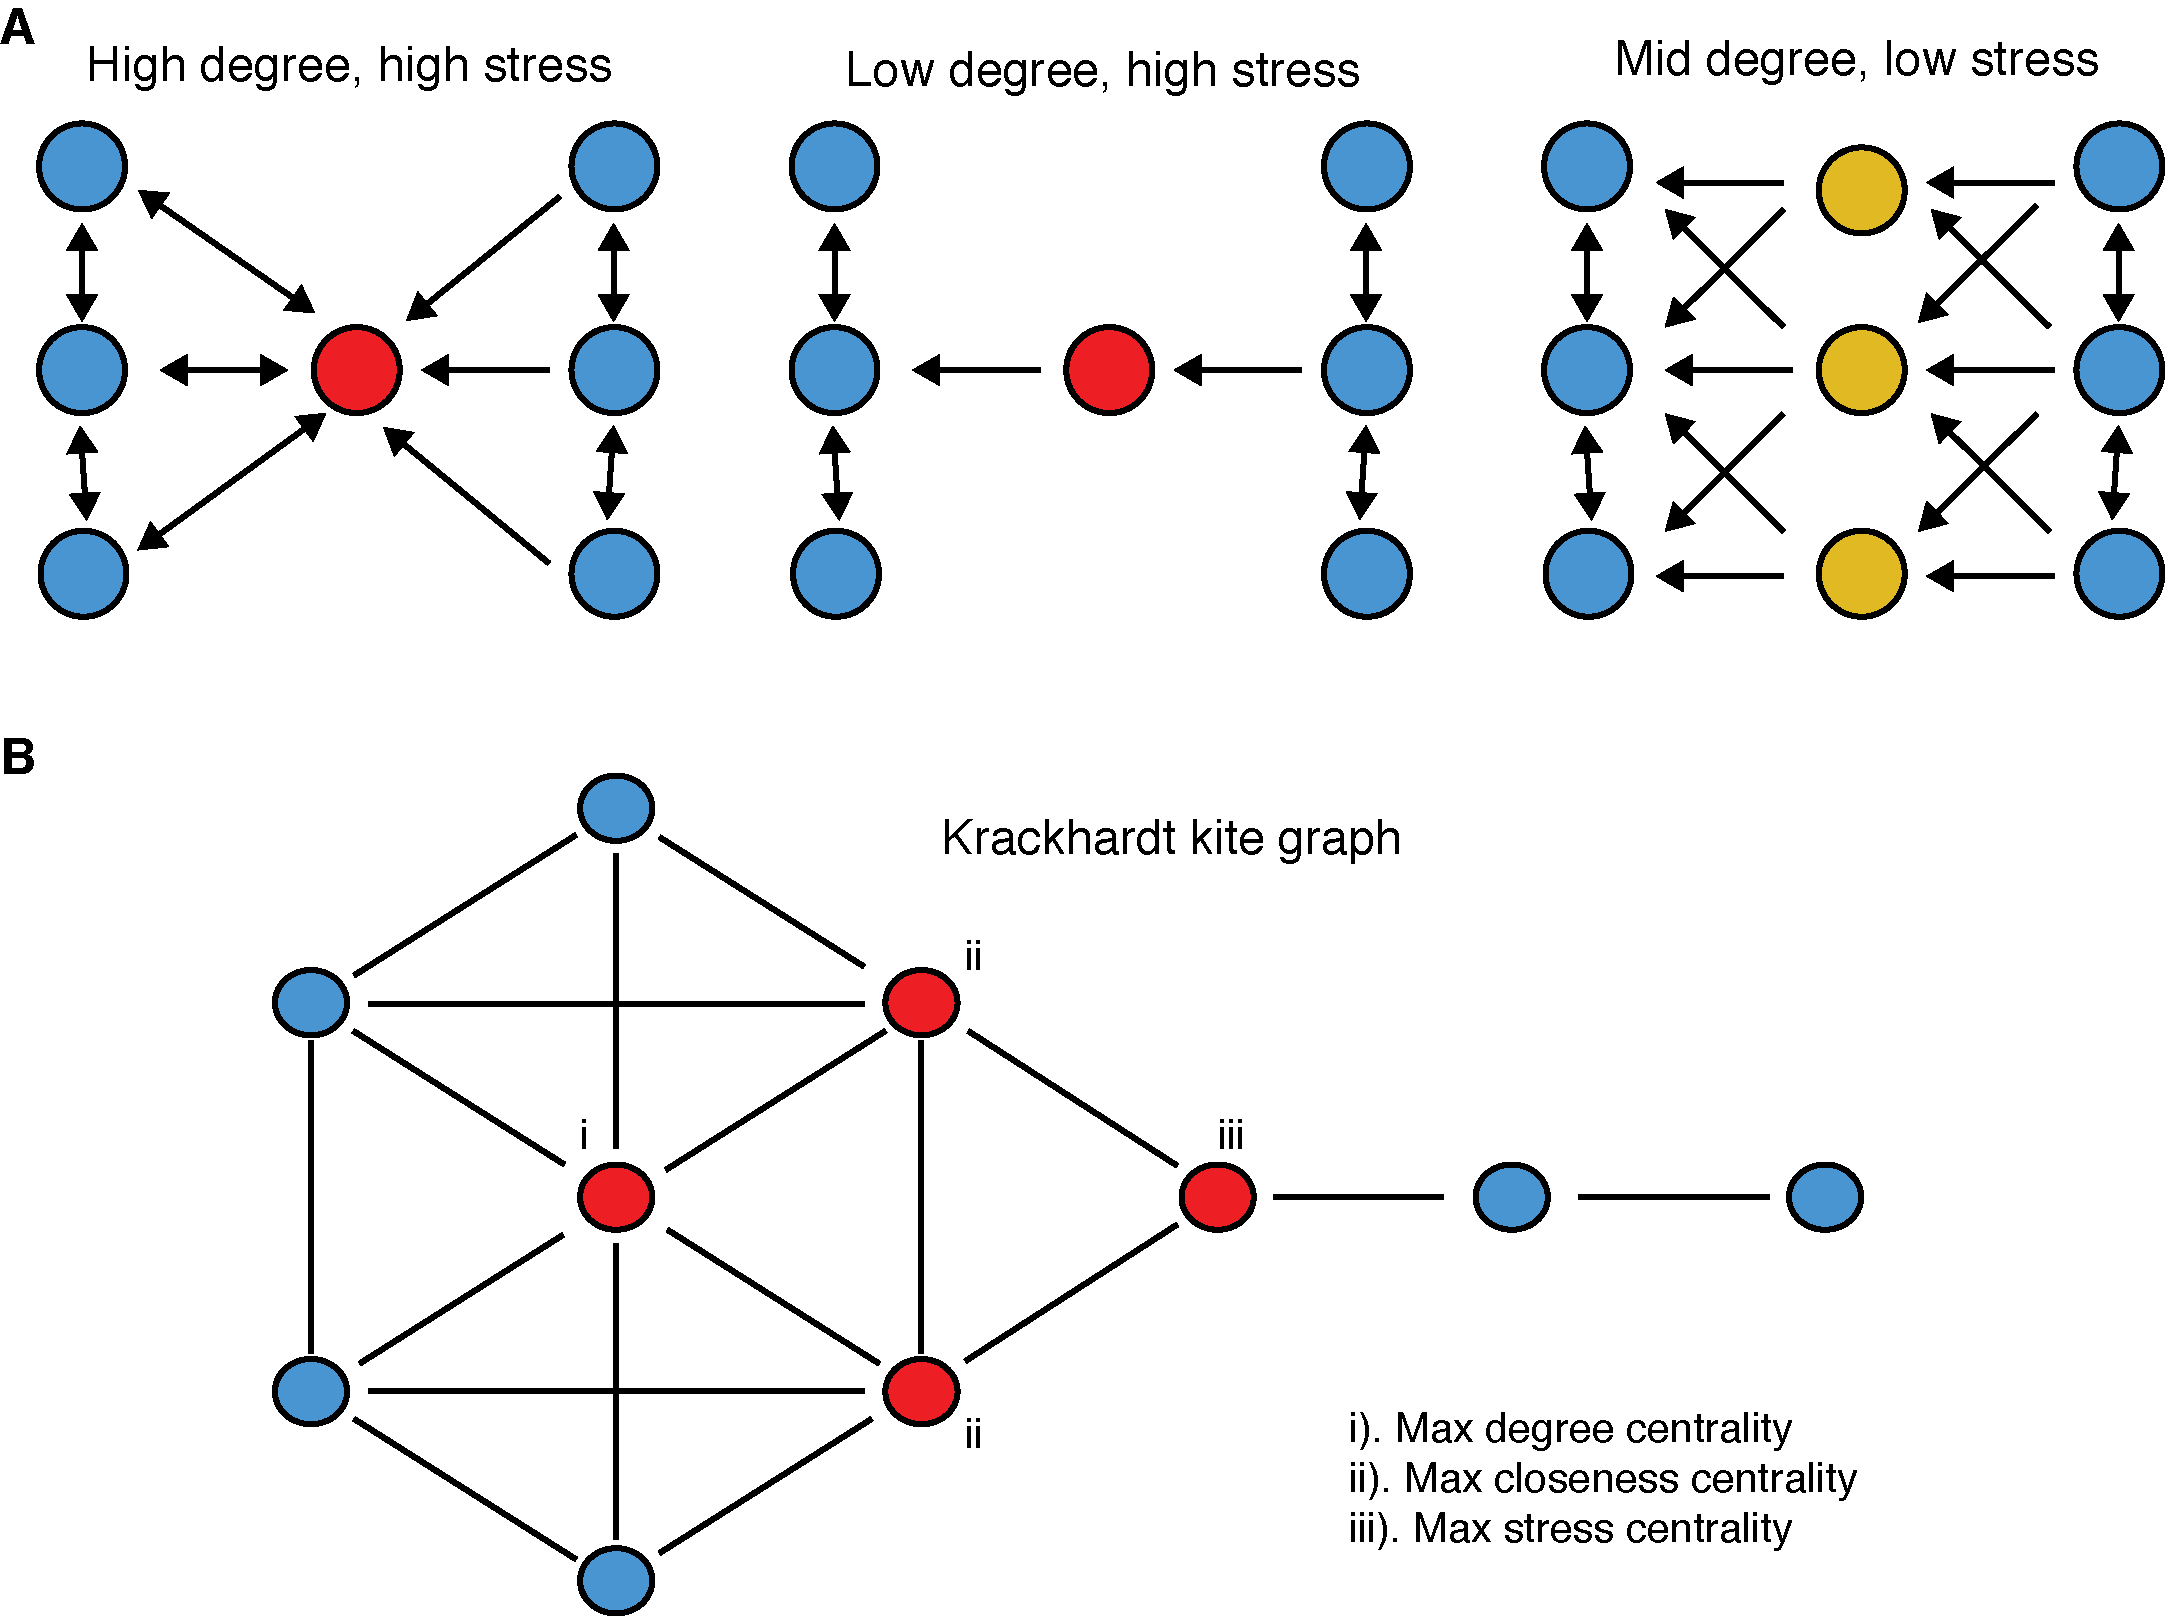
\includegraphics[width=\textwidth,height=\textheight,keepaspectratio]{figures/chapter1/ch1_centrality.png}
    \caption[{Illustration of network centrality measures.}]
    {\textbf{Illustration of network centrality measures.} 
    \textbf{(A)} Schematic of small example networks, exemplifying different levels of degree and stress centrality. Blue nodes are connected nodes in the networks, red and orange nodes are the measured NOIs. Red nodes display high centrality. Orange nodes display low/mid centrality. 
    \textbf{(B)} Krackhardt kite graph \citep{krackhardt_assessing_1990} illustrating how centrality measures emphasise different network structures.
    }
    \label{fig:ch1_stress-example}
\end{figure}

More advanced measures of centrality rely on the concept of "shortest paths". This is determined as the smallest possible number of nodes on a path between two other nodes. Closeness centrality is a measure that calculates the average number of shortest paths from the node of interest (NOI) to other nodes in the network \citep{bavelas_communication_1950}. This assumes that the most important nodes of a network must be generally close to all other nodes in a network. Measures related to this instead quantify how frequently the NOI is an intermediate of a shortest path between all other node pairs in a network. This measure can be represented as the total number of shortest paths (stress centrality), or the fraction of total shortest paths (betweenness centrality), as described in \cite{freeman_set_1977} (Fig. \ref{fig:ch1_stress-example}A). By this method, high stress or betweenness centrality nodes are assumed to exert greater control of communication between other nodes in the network. Different measures of centrality can emphasise different hubs of a network, as exemplified by the Krackhardt kite graph (Fig. \ref{fig:ch1_stress-example}B, \cite{krackhardt_assessing_1990}). Therefore, the choice of centrality measures can offer different conclusions. See Appendix \ref{fig:app_centrality-comparison} for the relationship between centrality measures.

The relevance of centrality measures in biological networks has been well-studied. For example, studies in \textit{S. cerevisiae}, \textit{C. elegans}, and \textit{D. melanogaster} have shown that high centrality can be associated with essential proteins \citep{hahn_comparative_2005, jeong_lethality_2001, koschutzki_centrality_2008}. \cite{hahn_comparative_2005} also noted that highly central proteins evolved more slowly. Interestingly, it has been suggested that nodes with low degree centrality but high stress centrality are more likely to represent nodes connecting distinct network modules (see Fig. \ref{fig:ch1_stress-example}A middle panel, \cite{joy_high-betweenness_2005, koschutzki_centrality_2008}). As such, combining centrality measures can reveal useful information on the structure of regulatory networks.

It is important to note that the networks these studies are based on are comparatively simple relative to mouse or human transcriptional networks, and so may not reflect essentiality as well in more complex organisms. Typically, while centrality is often a good indicator of network structure, it is not always a good indicator of essentiality. This is particularly true for TF models, as TF regulatory logic is complex with highly context dependent binding and function as well as regulatory redundancy (see section \ref{ch1:tf-structure-function}), that is difficult to capture in the GRN model itself. Nevertheless, investigating the centrality of TF hubs offers interesting insights into the complex structure of TF based networks.

\subsection{\label{ch1:grn-motifs}GRN motifs}

GRN models are a complex collection of data and observations. While centrality methods highlight specific regulatory hubs, they do not necessarily describe network structure. The Alon lab pioneered an approach to analysing GRNs by breaking graphs down into simple, repeating units \citep{shen-orr_network_2002, milo_network_2002, mangan_structure_2003}. This analysis focused on the identification of 3-4 node patterns, termed network motifs (or GRN motifs), that were enriched in biological networks. By describing networks in such a way, prominent GRN motifs can be probed whilst still preserving the small-scale structure of the network. Of particular note, these studies found one of the most prominently enriched GRN motifs in biological networks to be the feed-forward loop (FFL, Fig. \ref{fig:ch1_net-motifs}A, \cite{milo_network_2002, mangan_structure_2003}). Another recurring pattern, not specifically enriched in biological networks but important nonetheless, is the TF cascade (Fig. \ref{fig:ch1_net-motifs}B), in which a chain of TFs propagate signal to downstream targets \citep{lee_transcriptional_2002, rosenfeld_response_2003}. 

\begin{figure}[htbp]
    \centering
    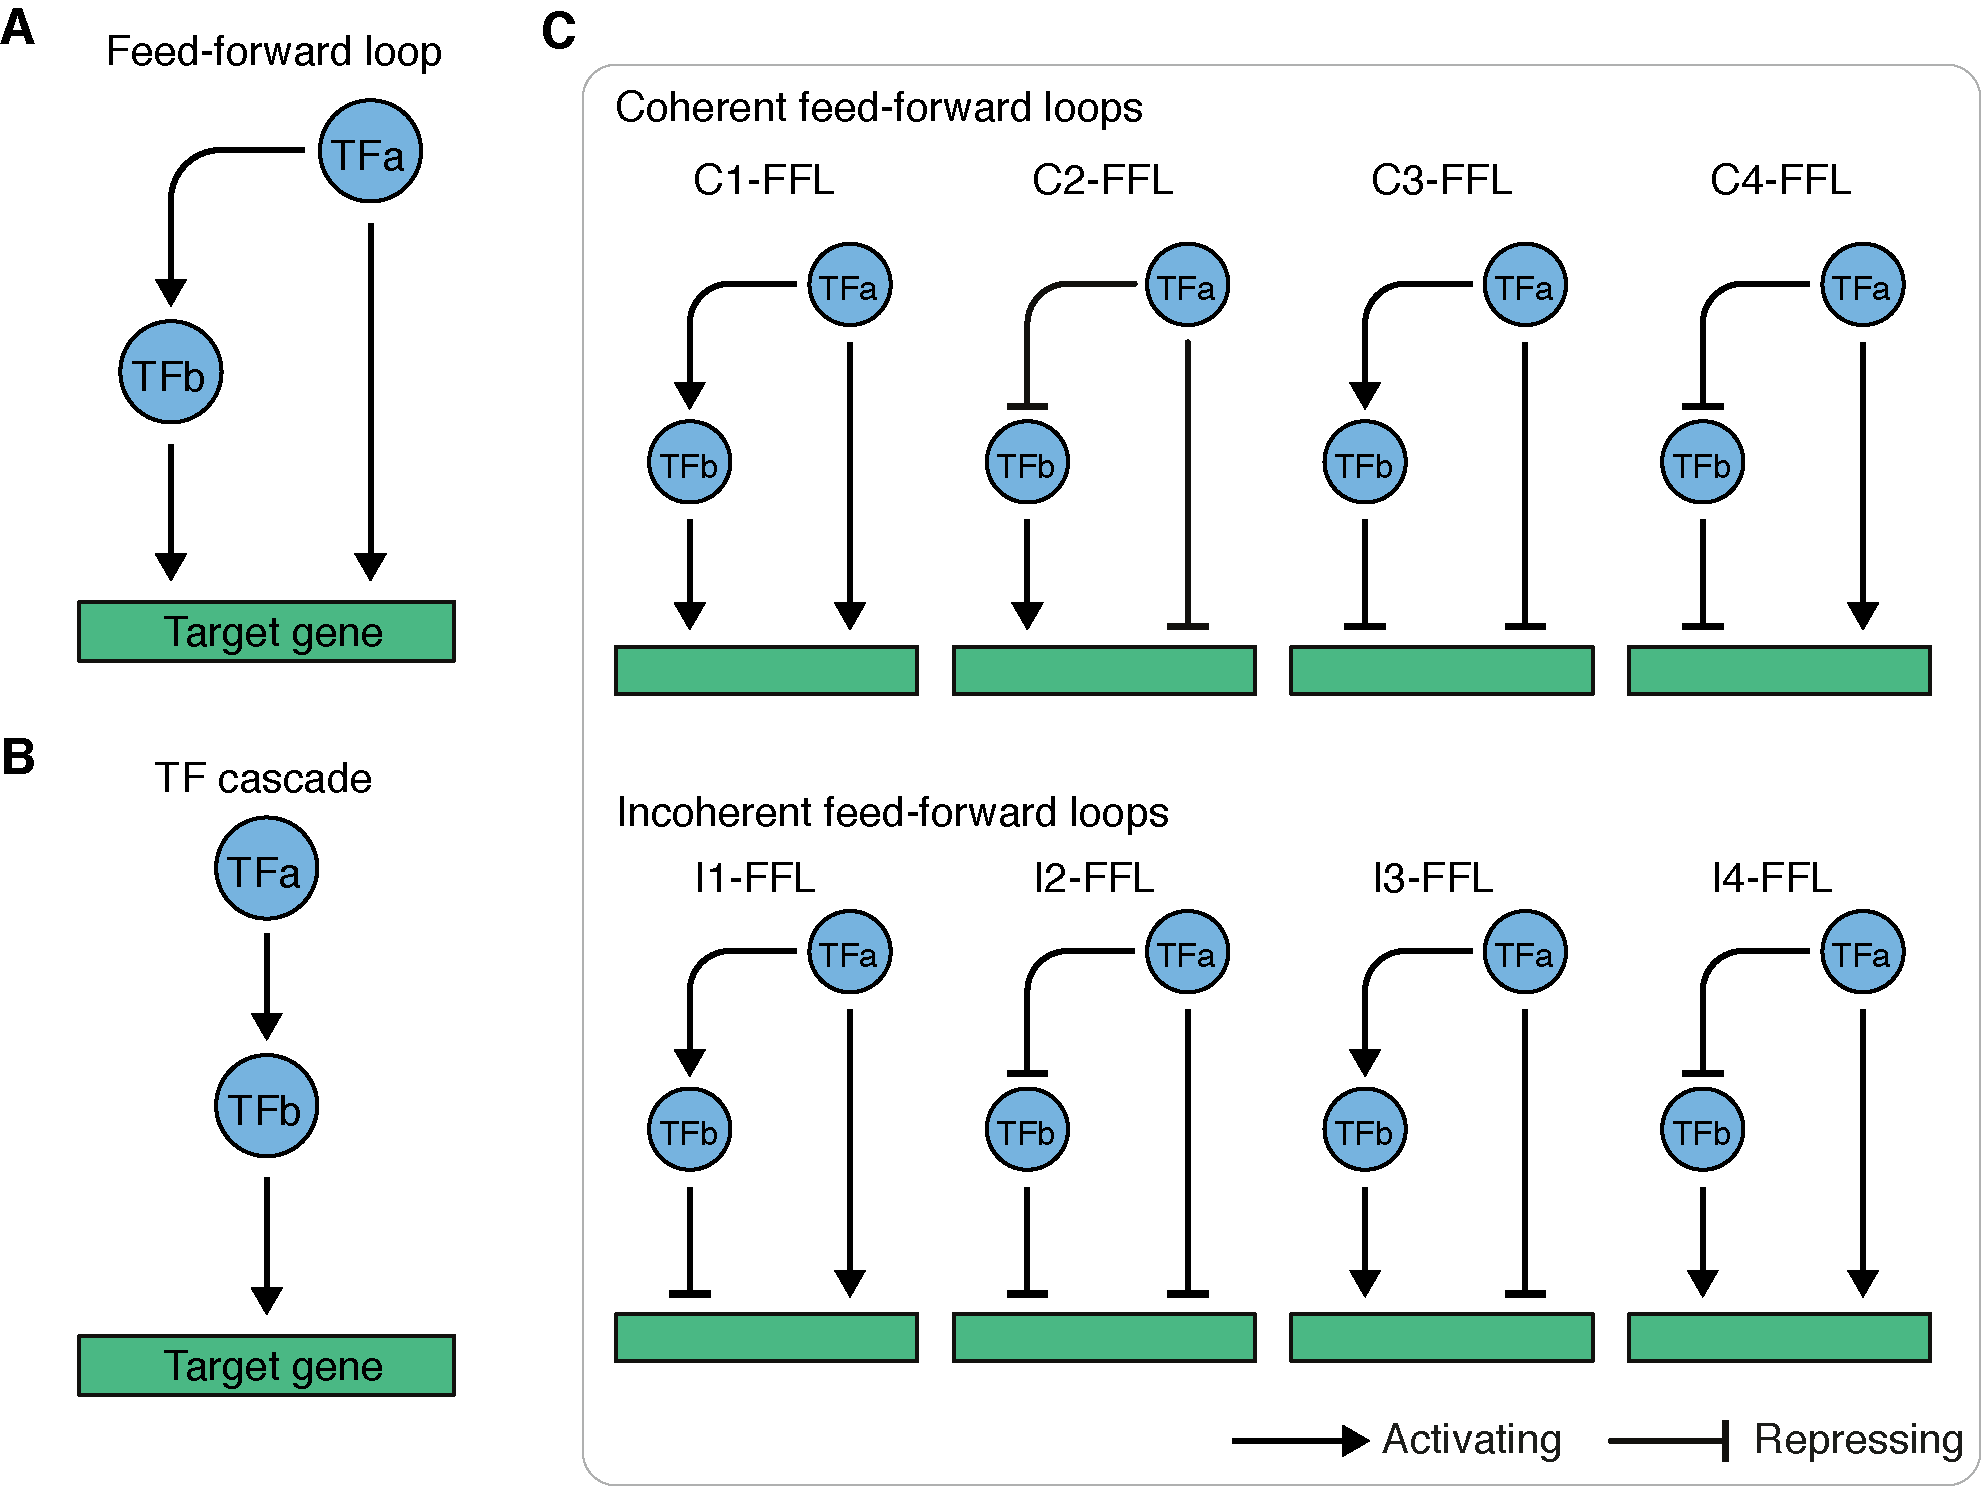
\includegraphics[width=\textwidth,height=\textheight,keepaspectratio]{figures/chapter1/ch1_net-motifs.png}
    \caption[{Illustration of network motifs.}]
    {\textbf{Illustration of network motifs.} 
    \textbf{(A)} Schematic of a FFL circuit.  
    \textbf{(B)} Schematic of a TF cascade. 
    \textbf{(C)} Schematic of coherent (top) and incoherent (bottom) FFL sub-types, determined by sign of effect for each interaction. 
    Blue nodes are TF regulators, green boxes are gene targets
    }
    \label{fig:ch1_net-motifs}
\end{figure}

Many publications have followed these analyses, focusing on the consequence of network structure on interaction dynamics \citep{goentoro_incoherent_2009, joanito_incoherent_2018, mangan_incoherent_2006, mangan_structure_2003}. The FFL can be divided into sub-types based on the sign of effect enacted by the TF regulators (Fig. \ref{fig:ch1_net-motifs}C, \cite{mangan_structure_2003}). This can be broadly grouped into two sub-types, where the regulatory logic of both TF regulators are the same (coherent) or opposite (incoherent). The C1-FFL and I1-FFL motifs (Fig. \ref{fig:ch1_net-motifs}C) were found to be particularly prevalent \citep{joanito_incoherent_2018, mangan_incoherent_2006}. These sub-types can be sub-divided further, as FFLs can be thought to function with AND/OR logic gates. Coherent FFL motifs that exhibit AND logic have been shown to be sign-sensitive delay elements, in that signal processing results in delayed activation going from an OFF to ON state, but rapid deactivation going from ON to OFF \citep{mangan_coherent_2003}. Coherent FFL motifs are also sign-sensitive, with a delay moving from an ON to OFF state \citep{kalir_coherent_2005}. The incoherent I1-FFL has been described as a pulse generator, where the repressive TF (TFb) has a strong effect on gene expression \citep{mangan_structure_2003, basu_spatiotemporal_2004}. This is described as TFa upregulating both TFb and the gene target, followed shortly after by TFb repression of the gene target. 

While GRN motifs are a useful tool for probing networks, and can offer insight into gene regulatory dynamics in small-scale circuits, it is important to acknowledge that these motifs do not always translate to biological function \citep{ingram_network_2006}. Like with measures of centrality, motif structure does not necessarily correlate with importance of a circuit, and to determine regulatory dynamics from GRN motifs detailed biochemical data is needed to support the model, which cannot reasonably be performed genome wide. Despite these drawbacks, GRN motifs are yet another method by which GRN models can be probed, and potentially elucidate key mechanisms of gene regulation.


\subsection{Model systems to apply network analyses}

In this thesis, I have investigated the use of GRN models for investigating the complex behaviour of TF regulation. The application of GRN models to haematopoiesis is an active and evolving field of research \citep{rothenberg_how_2021}. The diverse range of cell types and lineages, and complex transcriptional regulation involved in haematopoiesis makes this an ideal field to probe the use of TF GRNs. In particular, I aim to use GRNs to describe a process underlying the developmental origin of haematopoietic stem cells (HSCs) known as endothelial-to-haematopoietic transition (EHT) \citep{bertrand_haematopoietic_2010, boisset_vivo_2010, kissa_blood_2010} (see section \ref{ch1:eht}). This is a normal haematopoietic process, yet the disruption of normal circuits can sometimes drive disease. Therefore, I also aim to use GRNs to describe \textit{MLL}-rearranged leukaemias (see section \ref{ch1:mllr}), to investigate how normal transcriptional networks may be misregulated in disease. Importantly, EHT is dependent on the TF RUNX1 \citep{okuda_aml1_1996, wang_disruption_1996, north_cbfa2_1999, cai_haploinsufficiency_2000, chen_runx1_2009}, while \textit{MLL}-rearranged leukaemias can involve the overexpression of key TFs, such as \textit{RUNX1} and \textit{MYB}. Therefore, throughout this thesis I aim to anchor GRN analyses on the behaviour of two key TFs: RUNX1 and MYB.

%%%% Normal haematopoietic hierarchy %%%%

%\section{Normal haematopoietic hierarchy}

%Haematopoiesis is a hierarchical process, where all mature haematopoietic populations are derived from haematopoietic stem cells (HSCs).

%%%% Endothelial-to-haematopoietic transition %%%%

\section{\label{ch1:eht}The endothelial-to-haematopoietic transition}

\begin{wrapfigure}{r}{0.5\textwidth}
  \begin{center}
    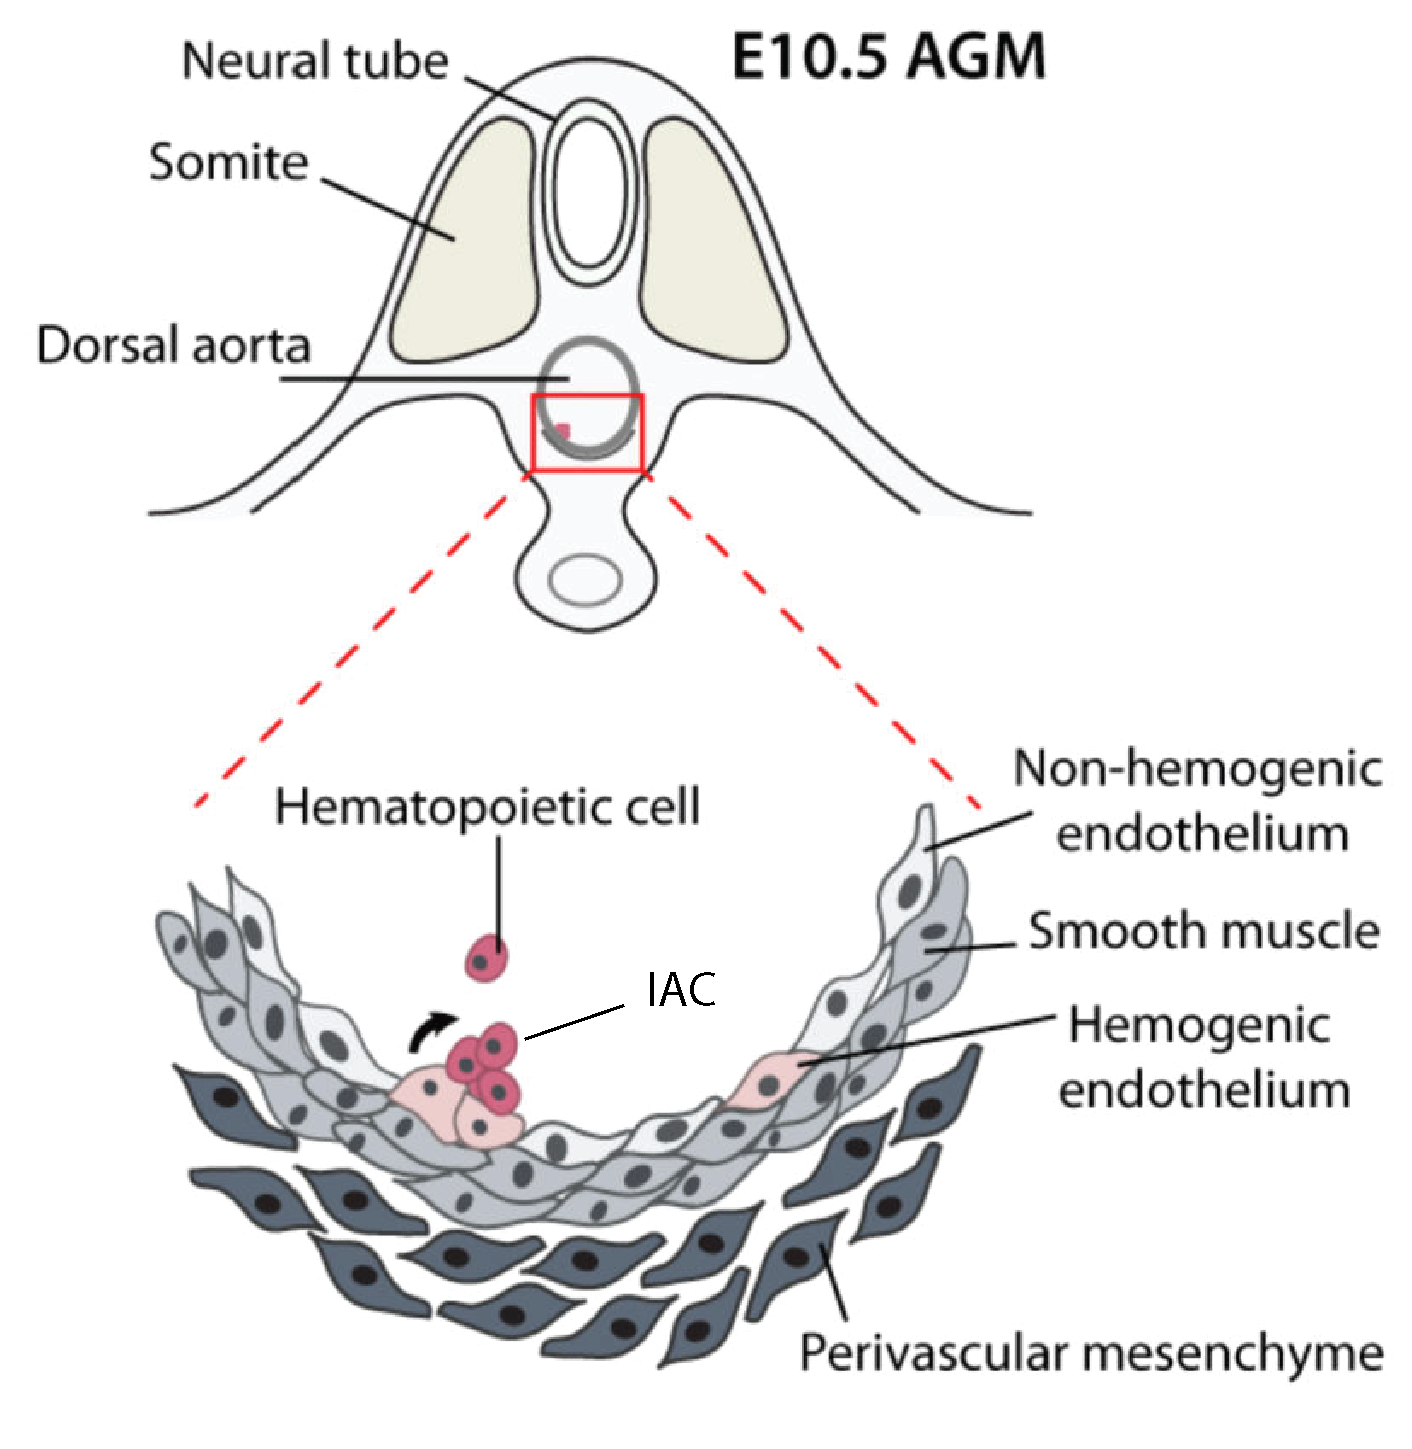
\includegraphics[width=0.48\textwidth]{figures/chapter1/ch1_swiers.png}
  \end{center}
  \caption[{Schematic of EHT at an E10.5 dorsal aorta.}]
    {\textbf{Schematic of EHT at an E10.5 dorsal aorta.} 
    Schematic of an E10.5 AGM, illustrating the EHT process. Boxed section magnified to highlight cell types. HE is coloured as pink, and haematopoietic cells and IACs as red. Non-HE endothelium is coloured as light grey, smooth muscles as mid grey, and mesenchymal cells as dark grey.
    \textit{Figure has been taken from \cite{swiers_short_2013}}.
    }
    \label{fig:ch1_swiers}
\end{wrapfigure}

The establishment of the haematopoietic system occurs in utero, and is a complex process that has been extensively explored in mice. In the embryo, haematopoiesis occurs broadly in three waves. The first, primitive, wave involves the generation of primitive erythroid progenitors originating at yolk sac blood islands from embryonic day E7.0 \citep{palis_development_1999, palis_yolk-sac_2001}. The second wave occurs from E8.25, generating erythro-myeloid progenitors, among others, in the yolk sac \citep{palis_development_1999, frame_erythro-myeloid_2013}. The final wave is established in E10.5 embryos, and occurs within the aorta-gonad-mesonephros (AGM) region at the embryonic dorsal aorta, generating the first adult-type HSCs \citep{medvinsky_definitive_1996, muller_development_1994, de_bruijn_definitive_2000}. The second and final waves establish definitive progenitors (originating from the yolk sac as well as the AGM) that persist into adult life \citep{yoshimoto_autonomous_2012, yoshimoto_embryonic_2011, gomez_perdiguero_tissue-resident_2015, gentek_hemogenic_2018}.

The initial establishment of haematopoietic stem and progenitor cells (HSPCs) occurs by a process referred to as endothelial-to-haematopoietic transition (EHT) \citep{bertrand_haematopoietic_2010, boisset_vivo_2010, kissa_blood_2010}. This process is best described in the embryonic dorsal aorta, but also occurs in the vitelline and umbilical (VU) arteries and the yolk sac \citep{north_cbfa2_1999, zovein_fate_2008, samokhvalov_cell_2007, padron-barthe_clonal_2014, mcgrath_distinct_2015}. It starts with the specification of a specialised subset of endothelial cells (EC) known as haemogenic endothelium (HE). Flat HE cells undergo transcriptional and morphological changes, and bud into the lumen of the dorsal aorta to form intra-aortic clusters (IACs) of cells (Fig. \ref{fig:ch1_swiers}) \citep{boisset_vivo_2010, bertrand_haematopoietic_2010, kissa_blood_2010, swiers_early_2013}. 

Runx1 is a master TF required for definitive haematopoiesis, and more specifically is critical for EHT to occur \citep{okuda_aml1_1996, wang_disruption_1996, north_cbfa2_1999, cai_haploinsufficiency_2000, chen_runx1_2009}. \textit{Runx1} expression begins in HE cells \citep{north_cbfa2_1999}, marking the start of, and commitment to, the haematopoietic program. Importantly, there is an enhancer 23 kb downstream (+23) of \textit{Runx1}, which was found to be a strong driver of reporter gene expression, and to mark both HE and IACs \citep{nottingham_runx1-mediated_2007, bee_nonredundant_2010, ng_runx1_2010}. This +23 enhancer is active in HE as early as E8.5, yet precedes endogenous \textit{Runx1} transcription at this stage \citep{swiers_early_2013}, suggesting the existence of a pre-HE population prior to commitment to the haematopoietic program. 

EHT has been well characterised as a number of specific intermediate cell states following \textit{Runx1} expression in HE, based on various markers and transcriptional profiles. HE and IAC cells undergo maturation through a series of well-defined cell states, classified by CD41, CD43, and CD45 cell surface markers \citep{taoudi_extensive_2008, rybtsov_hierarchical_2011, rybtsov_tracing_2014, ottersbach_endothelial--haematopoietic_2019}. HE first undergoes budding into the lumen of the dorsal aorta and differentiates into a pro-HSC state in E9.5 embryos, with a CD41\upos{}CD43\uneg{} phenotype \citep{rybtsov_tracing_2014}. From E10.5 to E11.5 these pro-HSCs then mature into pre-HSC type I cells with the expression of CD43, and subsequently pre-HSC type II cells with the expression of CD45 \citep{rybtsov_hierarchical_2011, taoudi_extensive_2008}. EHT can also be modelled in vitro, as mouse embryonic stem cells (mESCs) can be induced to differentiate into haematopoietic lineages \citep{galic_t_2006, carpenter_human_2011, woll_human_2009, lu_platelets_2011}, though it is important to highlight it closer represents yolk sac EHT, than dorsal aorta EHT \citep{mcgrath_distinct_2015}.

\subsection{Transcriptional regulation of EHT}

As cells mature through the various EHT states, dynamic transcriptional changes occur \citep{goode_dynamic_2016, ottersbach_endothelial--haematopoietic_2019, swiers_early_2013, solaimani_kartalaei_whole-transcriptome_2015, baron_single-cell_2018, zhu_developmental_2020, zeng_tracing_2019, bergiers_single-cell_2018, gao_transcriptional_2020, vink_iterative_2020, hou_embryonic_2020}. One example involves the Notch signalling pathway, where studies have shown that activation of Notch TFs leads to upregulated \textit{Gata2} and \textit{Runx1}, and subsequent HSC expansion \citep{burns_hematopoietic_2005, robert-moreno_rbpjkappa-dependent_2005, guiu_hes_2013}. While Notch activity is required for activation of essential TFs, it must also be restricted for the progression of pre-HSC I to pre-HSC II cells \citep{souilhol_developing_2016}, highlighting a requirement for tight temporal control of gene expression. Similarly, the TF Sox17 has been found to specify HE identity, yet is considered a repressor of Runx1 and Gata2 function and must be downregulated for EHT progression \citep{clarke_expression_2013, lizama_repression_2015, ottersbach_endothelial--haematopoietic_2019}. 

The regulation of \textit{Runx1} in EHT has been characterised by several studies. Multiple TFs, such as Meis1, Gata2, Tal1, and Ets factors, have been identified to regulate the +23 enhancer \citep{nottingham_runx1-mediated_2007, schutte_experimentally_2016}. Alongside Runx1, \textit{Gata2} expression is also important for the generation of HSCs through EHT, and has a further role in HSC maintenance \citep{tsai_early_1994, ling_gata-2_2004}. Runx1 has also been found to positively autoregulate itself, through interacting with the \textit{Runx1} P1 promoter \citep{martinez_transcriptional_2016}. Specifically within HE, \textit{Runx1} expression has been associated with the activity of genes involved in both cell adhesion and cell migration \citep{lie-a-ling_runx1_2014}, highlighting the potential for Runx1 to drive the morphological changes underpinning the HE budding process. Further, Runx1 is known to upregulate expression of the \textit{Gfi1} and \textit{Gfi1b} TFs, which subsequently leads to a Gfi1/Gfi1b mediated loss of endothelial identity \citep{wilson_gfi1_2010, lancrin_gfi1_2012}. This activity is essential for HE to undergo morphological changes, and is a requirement for haematopoietic development. Runx1 is also well characterised to activate \textit{Spi1} (which encodes PU.1) \citep{huang_pu1_2008}, an essential regulator of later haematopoietic populations that drives myeloid lineage commitment \citep{imperato_runx1pu1_2015}.
 
EHT involves diverse transcriptional changes across several cell type intermediates, and as Runx1 is such an important TF for this to occur, this makes for an exciting system in which to test a GRN model and investigate the role of the Runx1 TF.


\section{\label{ch1:mllr}\textit{MLL}-rearranged leukaemia}

\begin{figure}[!t]
    \centering
    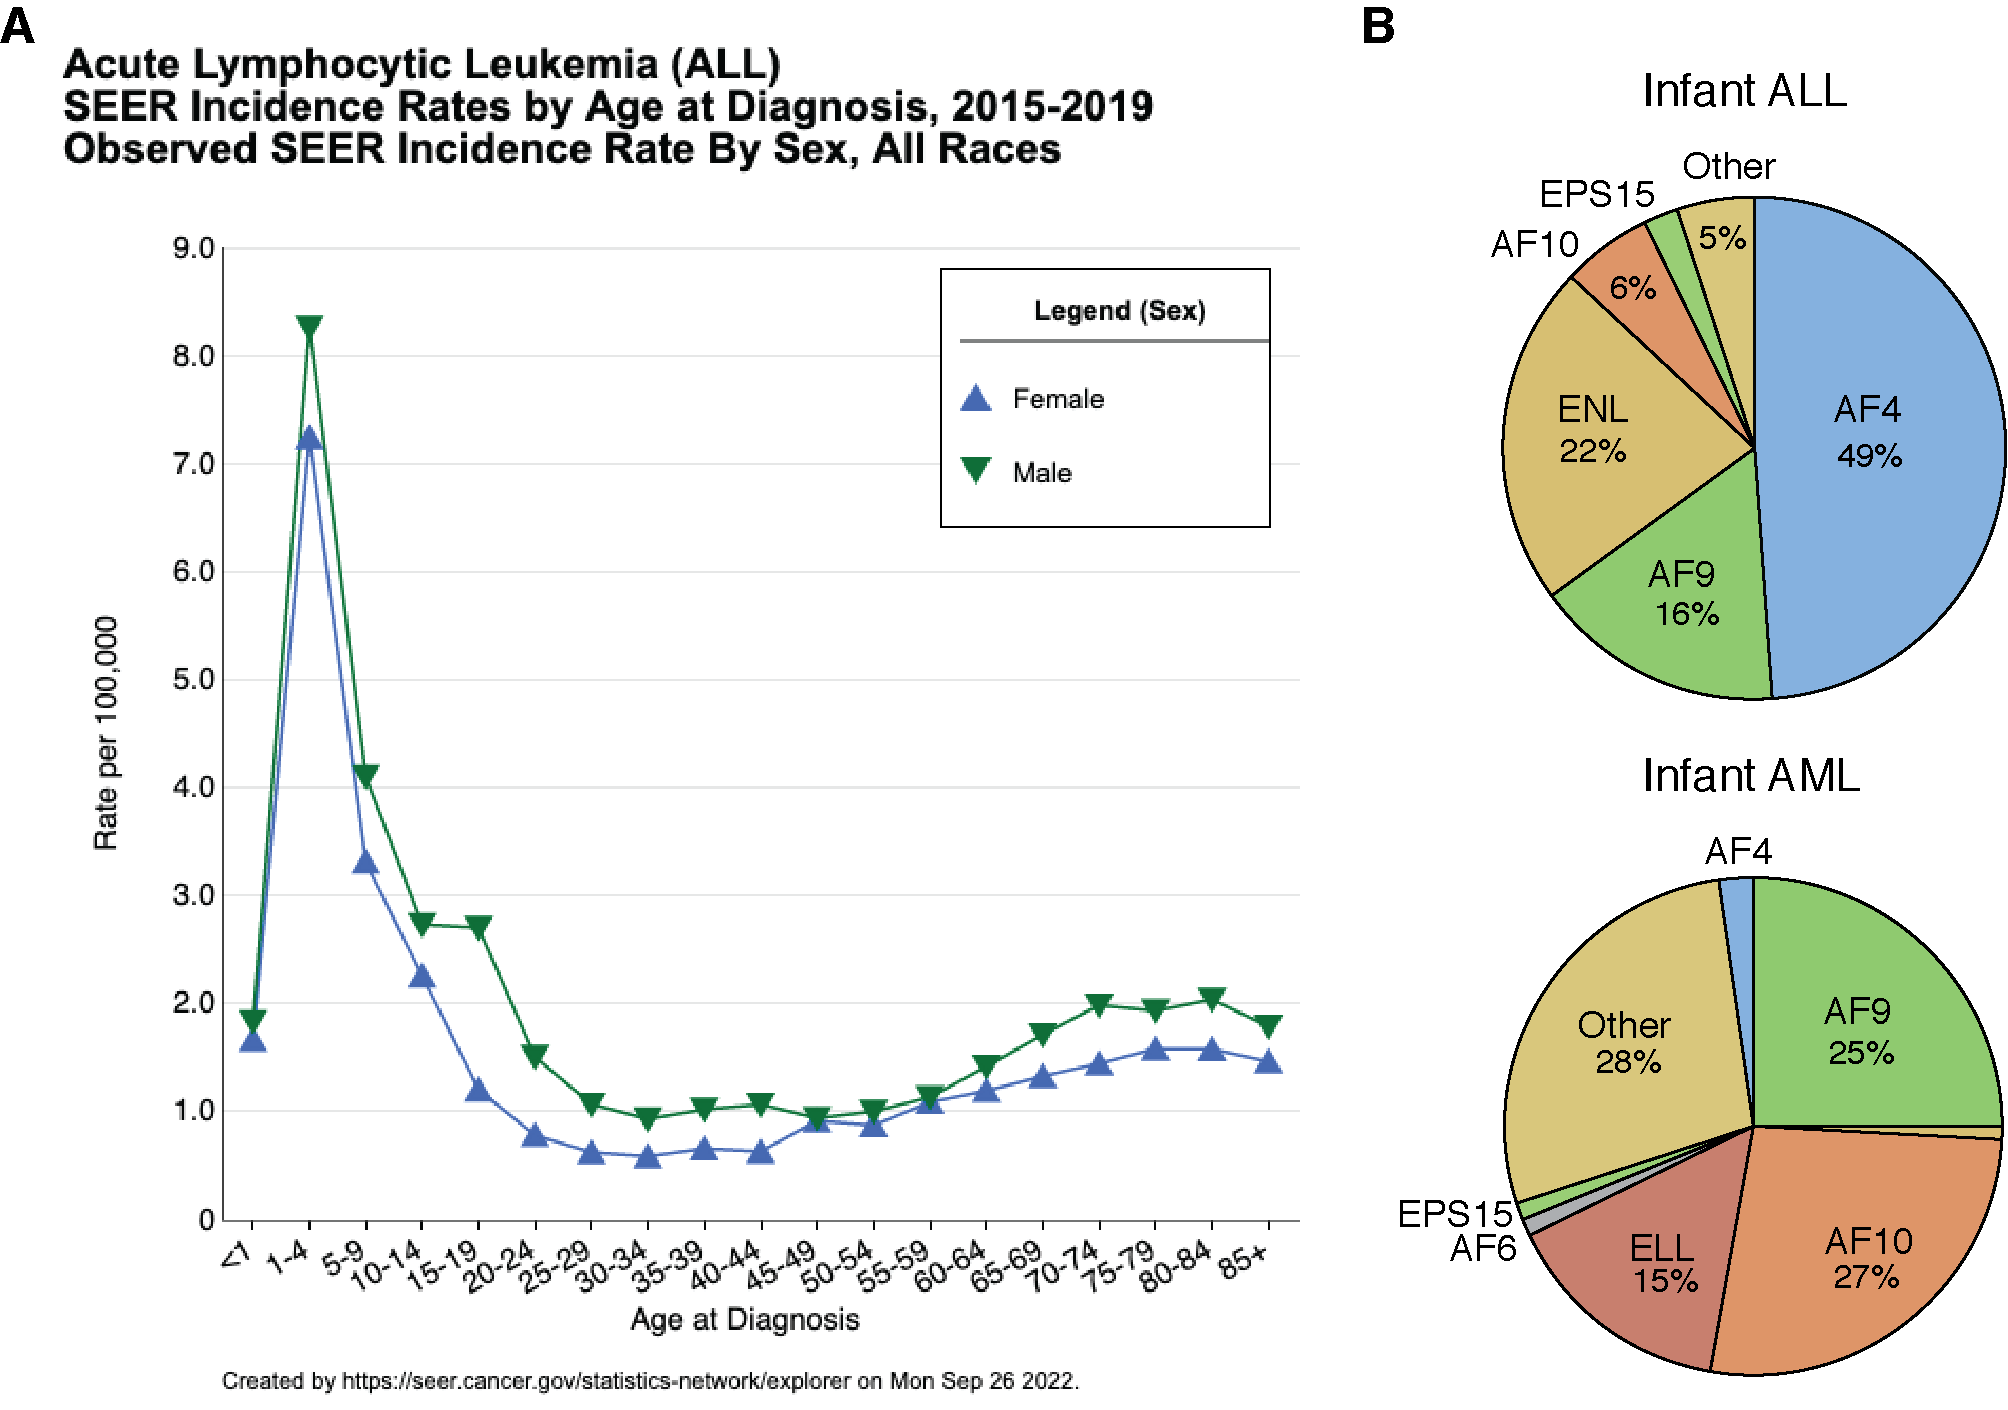
\includegraphics[width=\textwidth,keepaspectratio]{figures/chapter1/ch1_all-incidence.png}
    \caption[{Incidence of ALL and infant \textit{MLL}r fusion partners.}]
    {\textbf{Incidence of ALL and infant \textit{MLL}r fusion partners.} 
    \textbf{(A)} ALL incidence rates by age, based on data collected between 2015 and 2019. \textit{Data and image sourced from the National Cancer Institute (NIH) Surveillance Epidemiology and End Results (SEER) programme \citep{national_cancer_institute_seerexplorer_2022}}. 
    \textbf{(B)} Frequency of \textit{MLL} fusion partners in \textit{MLL}r infant ALL and AML. \textit{Figure adapted from \cite{meyer_mll_2018}}. 
    }
    \label{fig:ch1_all-incidence}
\end{figure}

Leukaemia is a cancer of the blood, of which there are multiple subtypes. Two prevalent subtypes of leukaemia are acute myeloid leukaemia (AML) and acute lymphoblastic leukaemia (ALL). These diseases can affect both young and old people alike, with ALL maintaining a particularly high prevalence in children (Fig. \ref{fig:ch1_all-incidence}A, \cite{national_cancer_institute_seerexplorer_2022, meyer_mll_2018}). Large strides have been made in curing both childhood ALL and AML, however infant leukaemias (patients < 1 year of age) are still associated with a dismal prognosis \citep{rice_mll-rearranged_2020, pieters_outcome_2019}. A particular characteristic of infant leukaemias is the frequency of chromosomal rearrangements at the \textit{Mixed-Lineage Leukemia} (\textit{MLL}, also known as \textit{KMT2A}) gene. These chromosome translocations fuse \textit{MLL} in frame to one of a wide number of partner genes, creating novel fusion proteins (MLL-FPs). While only 10\% of acute leukaemias across all ages carry \textit{MLL} rearrangements (\textit{MLL}r), this frequency rises to 70\% in infant leukaemias \citep{meyer_mll_2013, mann_improved_2010, winters_mll-rearranged_2017, muntean_pathogenesis_2012}. \textit{MLL}r is associated with a poor prognosis, with a 20-40\% 5 year event-free survival, compared to > 60\% in wild-type \textit{MLL} (wt-\textit{MLL}) \citep{winters_mll-rearranged_2017, hilden_analysis_2006, tomizawa_outcome_2007}. Additionally, \textit{MLL}r leukaemias respond poorly to treatment, and 50-60\% of \textit{MLL}r leukaemias in remission result in relapse \citep{winters_mll-rearranged_2017, reaman_treatment_1999, milne_mouse_2017}. There is a clear clinical need to investigate \textit{MLL}r leukaemias, due to the prevalence and severity in infant patients, as well as its resistance to treatment strategies.

Rearrangements of the \textit{MLL} gene can result in translocations with a wide range of partner genes, resulting in unique fusion proteins. In \textit{MLL}r infant ALL (iALL), the most common fusion is between \textit{MLL} and \textit{AF4}, resulting in an MLL-AF4 fusion protein (Fig. \ref{fig:ch1_all-incidence}B, Fig. \ref{fig:ch1_mll-rearrange}A, \cite{meyer_mll_2018}). Conversely, in \textit{MLL}r infant AML, \textit{AF4} is a relatively rare, with \textit{ELL}, \textit{AF10}, and \textit{AF9} accounting for 67\% of \textit{MLL} fusion partners. There are also cases where MLL-AF4 iALLs relapse after treatment, arising as an AML derived from the original leukaemic clone \citep{dorantes-acosta_lineage_2012, gardner_acquisition_2016}. This suggests that while different fusion partners are biased to specific lineages, a single fusion protein can drive both ALL and AML phenotypes.

\subsection{\label{ch1:mll-af4-function}Structure and function of the MLL fusion protein complex}

MLL is an important developmental protein, particularly for haematopoiesis \citep{mcmahon_mll_2007, crump_why_2019}. MLL is a methyltransferase that methylates histone H3 lysine 4, and this activity is driven through its SET domain, which was found to be important for wt-MLL upregulation of \textit{Hox} genes \citep{milne_mll_2002, nakamura_all-1_2002}. \textit{MLL} translocations involve the fusion of N-terminus MLL to the C-terminus of a partner protein, resulting in loss of the SET domain and wt-MLL methyltransferase activity (Fig. \ref{fig:ch1_mll-rearrange}B, \cite{winters_mll-rearranged_2017, zeleznik-le_11q23_1994}). However, the DNA binding activity of wt-MLL is mostly harboured within the N-terminus, and as such MLL binding affinities strongly direct binding of the MLL-FP \citep{winters_mll-rearranged_2017, zeleznik-le_11q23_1994}. This consists of a CxxC domain, which binds unmethylated CpG (uCpG) islands \citep{birke_mt_2002}, as well as multiple AT-hooks that promote binding to AT-rich DNA \citep{zeleznik-le_11q23_1994} (Fig. \ref{fig:ch1_mll-rearrange}B). DNA binding is also thought to be driven through N-terminal MLL recruitment of Menin, and subsequently LEDGF, as LEDGF binds H3K36me2 marks \citep{hughes_menin_2004, milne_menin_2005, yokoyama_menin_2008, zhu_ash1l_2016}, though this has been shown to be dispensable for targeting to the \textit{HOXA9} gene \citep{milne_multiple_2010}. The C-terminus of wt-MLL also contains multiple plant homeodomain (PHD) fingers and a bromodomain that contribute to chromatin binding (Fig. \ref{fig:ch1_mll-rearrange}B), and are lost in the MLL-FP \citep{zeleznik-le_11q23_1994}.

\begin{figure}[htbp]
    \centering
    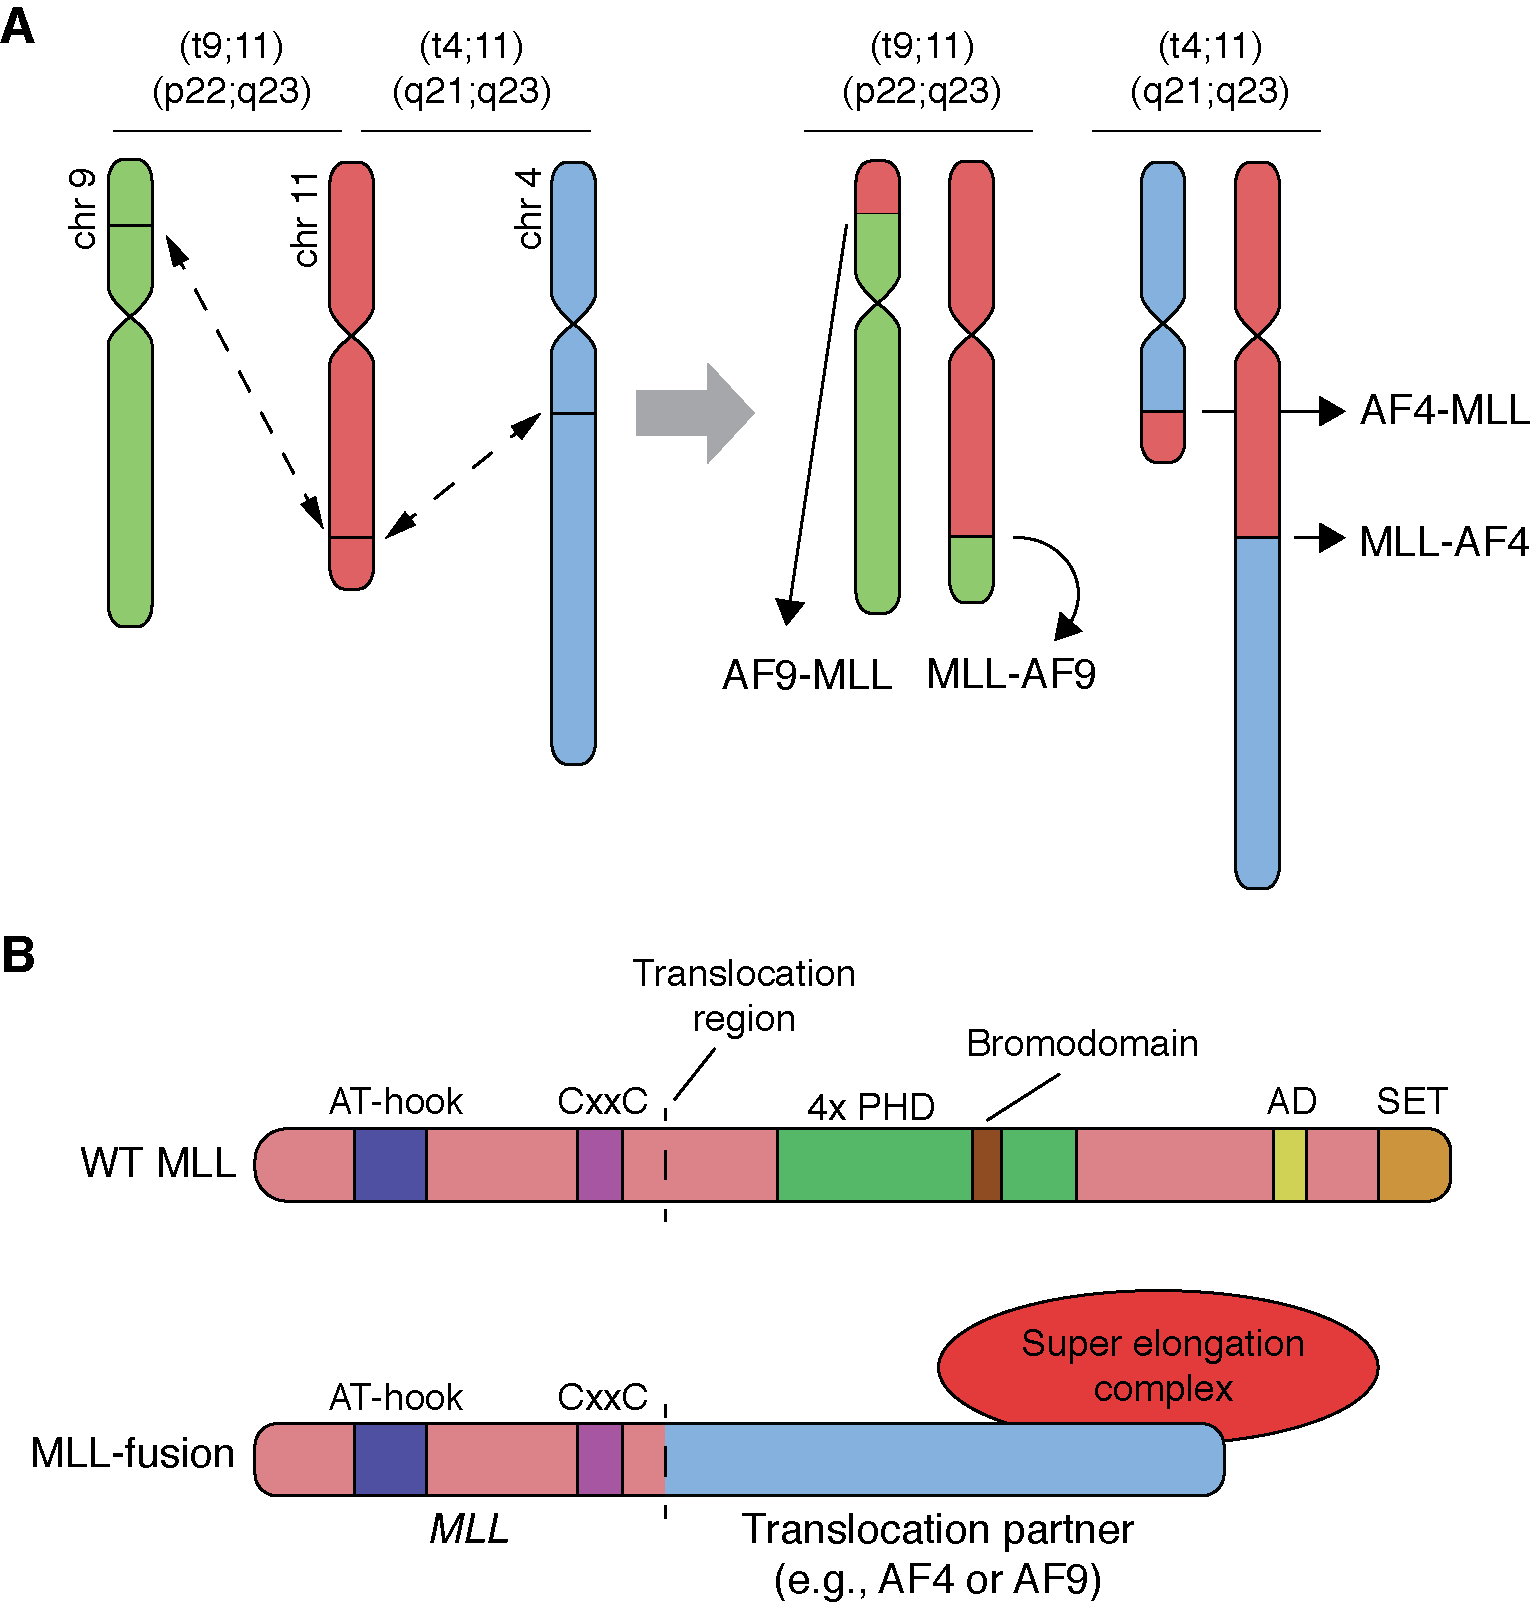
\includegraphics[width=0.8\textwidth,keepaspectratio]{figures/chapter1/ch1_mll-rearrange.png}
    \caption[{Schematic of \textit{MLL} translocations, and wild type and MLL fusion protein structure.}]
    {\textbf{Schematic of \textit{MLL} translocations, and wild type and MLL fusion protein structure.} 
    \textbf{(A)} Schematic of the chromosomal rearrangements resulting in MLL-AF4 and MLL-AF9 fusion proteins. \textit{MLL} is located on chromosome 11, and \textit{AF4} and \textit{AF9} are located on chromosome 4 and 9, respectively. Horizontal black lines on chromosomes indicate the translocation break points. Dashed lines indicate translocation. 
    \textbf{(B)} Simplified schematic of MLL fusion protein structure, adapted from \cite{winters_mll-rearranged_2017}.
    }
    \label{fig:ch1_mll-rearrange}
\end{figure}

Both MLL-AF4 and MLL-AF9 fusion proteins drive transcription through the recruitment of various factors, driven through the AF4 or AF9 C-terminus. Importantly, this includes the recruitment and assembly of a super elongation complex (SEC) that drives gene transcription (Fig. \ref{fig:ch1_mll-rearrange}B), consisting of both AF4 and AF9, as well as AFF4, ENL, ELL1, ELL2, and ELL3, among others \citep{lin_aff4_2010, smith_super_2011, lin_dynamic_2011, ballabio_molecular_2012, takahashi_molecular_2020, slany_mll_2020, yokoyama_higher-order_2010}. This complex contains multiple common MLL fusion partners, and as such highlights how different MLL-FPs can have similar behaviours by recruiting a similar overall complex. The MLL-FP complex also recruits Disruptor of Telomeric Silencing 1-like (DOT1L) \citep{bernt_mll-rearranged_2011, biswas_function_2011, lacoste_disruptor_2002, milne_leukemogenic_2005, okada_hdot1l_2005, mueller_role_2007, slany_mll_2020, lin_instructive_2016, krivtsov_h3k79_2008}, which is a methyltransferase for H3 lysine 79 (H3K79) \citep{steger_dot1lkmt4_2008}. H3K79 methylation has been associated with strong transcriptional overexpression at a subset MLL-FP targets, such as \textit{HOXA9} and \textit{RUNX1}, and perturbation of DOT1L activity significantly downregulates gene expression \citep{kerry_mll-af4_2017, godfrey_dot1l_2019, milne_leukemogenic_2005, wilkinson_runx1_2013}. Additionally, in \textit{MLL}r leukaemia H3K79me is also found enriched at a subset of intragenic enhancers, and maintains enhancer-promoter (E-P) interactions \citep{godfrey_dot1l_2019}. A related cofactor that is associated with the MLL-FP complex, though not directly recruited, is BRD4. BRD4 binds acetylated chromatin via its bromodomain \citep{dey_double_2003}, but in addition to this it was found that BRD4 was associated with members of the SEC, and further that BRD4 was a potential therapeutic target for MLL-AF9 leukaemias \citep{dawson_inhibition_2011, zuber_rnai_2011}. BRD4 directly interacts with P-TEFb and stimulates transcription by increasing P-TEFb dependent Pol II phosphorylation \citep{yang_recruitment_2005, jang_bromodomain_2005}. It has also been reported that DOT1L and BRD4 functionally cooperate in MLL leukaemias, through EP300 acetylating H4K5 at methylated H3K79 regions, and subsequent BRD4 recruitment to the acetylated chromatin \citep{gilan_functional_2016}. 

An interesting feature of MLL-FPs, most characterised with MLL-AF4, is the observation that at a subset of gene targets MLL-AF4 binds to uCpG promoters then spreads into the gene body \citep{kerry_mll-af4_2017}. These "spreading targets" are highly overexpressed, and spreading is associated with enriched Menin and H3K79 methylation. Interestingly, these overexpressed targets were also highly susceptible to DOT1L inhibition, highlighting DOT1L as key driver at this subset of targets.

\subsection{Transcriptional impact of MLL fusion proteins}

As MLL-AF4 and MLL-AF9 recruit a SEC, and are associated with transcriptional coactivators (i.e., BRD4), these fusion proteins are considered to act as drivers of gene transcription rather than repressors. Interestingly, \textit{MLL}r leukaemias are associated with few or no cooperating mutations \citep{andersson_landscape_2015, the_cancer_genome_atlas_research_network_genomic_2013, bardini_dna_2010, bardini_implementation_2011}, suggesting that the MLL fusion protein alone is sufficient to drive leukaemogenesis. In fact, numerous studies have shown that expression of MLL-AF4 or MLL-AF9 is sufficient to induce leukaemia \citep{rice_human_2021, krivtsov_h3k79_2008, krivtsov_cell_2013}. As MLL fusion proteins function by overexpressing genes, and are sufficient on their own for leukaemogenesis, \textit{MLL}r leukaemias may be considered to be an entirely transcriptionally driven disease. This makes for an ideal system to probe aberrant gene expression profiles with a GRN approach.

\textit{BCL2} is an MLL-AF4 and MLL-AF9 target of particular importance. It has been reported that not only does MLL-AF4 bind to the \textit{BCL2} promoter, but also a downstream enhancer, resulting in overexpression of the gene \citep{godfrey_mll-af4_2017, benito_mll-rearranged_2015}. MLL-AF4 leukaemias are highly sensitive to \textit{BCL2} perturbation \citep{robinson_abundant_2008}, in keeping with the role of BCL-2 in deterring apoptosis \citep{czabotar_control_2014, singh_regulation_2019}. This highlighted \textit{BCL2} as a key gene in cell survival. As such, venetoclax, a drug targeting BCL-2 protein, has been a successful treatment of MLL-AF4 leukaemias \citep{benito_mll-rearranged_2015, khaw_venetoclax_2016, niu_acute_2014}. 

MLL-AF4 and MLL-AF9 have also been found to overexpress \textit{MYC}, a TF and oncogene that drives proliferation \citep{dang_myc_2012, prange_mll-af9_2017}. \textit{MYC} overexpression typically results in apoptosis, either through indirectly activating p53 (p53-dependent) or modulating the balance between pro-apoptosis and anti-apoptotic factors (p53-independent) \citep{fairlie_co-operativity_2021}. However, the overexpression of \textit{BCL2} prevents activation of the p53-independent apoptotic pathway, allowing MLL-AF4 and MLL-AF9 to upregulate \textit{MYC} and increase proliferation. \citep{fairlie_co-operativity_2021, fanidi_cooperative_1992, bissonnette_apoptotic_1992}. As such, both \textit{BCL2} and \textit{MYC} must be expressed for the full leukaemic potential of \textit{MLL}r leukaemias.

Another key gene is \textit{PROM1} (encoding CD133 protein), which is an MLL-AF4 spreading target that is important for leukaemic growth \citep{kerry_mll-af4_2017, mak_mixed_2012, godfrey_h3k79me23_2021}. Interestingly, it was found that not only does MLL-AF4 drive expression through the promoter, but H3K79 methylation deposited by DOT1L at an intragenic enhancer was found to maintain E-P interactions, potentially enhancing promoter activity \citep{godfrey_h3k79me23_2021}. Further, this intragenic enhancer also interacted with a nearby gene \textit{TAPT1}, highlighting the capacity for complex regulation driven by MLL-AF4, not just through promoter binding, but modulation of enhancer activity and E-P interactions.

RUNX1 and MYB are two TFs of particular interest. \textit{RUNX1} is overexpressed in MLL-AF4 ALL leukaemia, and is an MLL-AF4 spreading target \citep{wilkinson_runx1_2013, kerry_mll-af4_2017}. It has also been found that \textit{RUNX1} perturbation is detrimental for leukaemic growth \citep{wilkinson_runx1_2013}. While RUNX1 itself is a potent transcriptional regulator, \cite{wilkinson_runx1_2013} suggested an additional regulatory mechanism whereby RUNX1 interacts with the AF4-MLL (the reciprocal fusion protein of MLL-AF4) complex. MYB is a known to be upregulated by MLL-AF9 in MLL-AF9 AML, after which these AML become addicted to MYB \citep{zuber_integrated_2011}. Both RUNX1 and MYB are expressed in numerous haematopoietic populations, in addition to the critical role of RUNX1 in EHT (section \ref{ch1:eht}), and are important regulators of several lineages \citep{ichikawa_role_2013, wang_myb_2018}. Probing the activity of these deregulated TFs in leukaemia will be important to fully understand the regulation of these diseases, as well as how aberrantly expressed transcriptional networks contribute to leukaemogenesis.

\section{Thesis overview and aims}

In this thesis I have focused on the application of GRN models to investigate gene regulation in a normal developmental process, and gene regulation in aberrantly regulated processes, most notably leukaemia. Gene regulation is complex to model in vivo, and TFs add a layer of complexity that is difficult to address. The specific combination of TFs, not just expressed in a cell but bound at a specific genomic locus, can drastically alter regulatory output. This specific combinatorial code underpins all developmental processes, can drive change in cell identity, and can be a critical component for understanding how diseases are driven.

Haematopoiesis involves complex gene regulation and multiple lineages, and cell identity is relatively plastic, with cells capable of being reprogrammed into different lineages \citep{schutte_experimentally_2016, riddell_reprogramming_2014, batta_direct_2014}. As a result, it is also an active field of research for applying GRN models \citep{rothenberg_how_2021}. EHT is a particularly interesting process associated with the developmental origin of HSCs, that requires dose-specific and temporally controlled activation of TFs and dynamic regulation of gene expression. However, the disruption of normal regulatory processes can result in disease, as seen with \textit{MLL}r acute leukaemias. MLL-AF4 and MLL-AF9 leukaemias are interesting haematopoietic malignancies, that are unique in being driven by a single translocation event and are a transcriptional disease \citep{andersson_landscape_2015, the_cancer_genome_atlas_research_network_genomic_2013, bardini_dna_2010, bardini_implementation_2011, rice_human_2021, krivtsov_h3k79_2008, krivtsov_cell_2013}. 

The well-defined populations of EHT and dynamic gene regulation make for a promising system to probe using GRN approaches. As the RUNX1 TF is critically required for EHT, it is a pivotal TF to investigate in this GRN. \textit{RUNX1} is also an important MLL-AF4 target overexpressed in \textit{MLL}r ALL, and as such \textit{MLL}r leukaemias represent a system in which RUNX1 behaviour can be studied within a misregulated, leukaemic GRN. Studying GRN models of these systems offers an interesting view of RUNX1 behaviour in different contexts: normal and aberrant haematopoiesis. MYB is also an interesting TF that, while not critical for EHT, is an essential overexpressed gene MLL-AF9 AML. Studying GRN models with a view of RUNX1 and MYB behaviour, with a particular focus on how these TFs cooperate with other regulators, will offer interesting comparisons.
%\clearpage

\noindent
There are three questions central to this thesis project: 

\vspace*{-5mm}
\begin{enumerate}
    \item What novel regulatory mechanisms underpinning key processes can be understood using GRN models?
    \item What insight into TF combinatorial logic and regulatory synergy driving processes do these GRNs offer?
    \item How are normal transcriptional networks deregulated in \textit{MLL}r leukaemia?
\end{enumerate}

\vspace*{-5mm}
I have established and explored a model of EHT regulation in chapter \ref{chapter3_EHT} to investigate key regulatory interactions involving Runx1, and to probe cases of TF cooperation that may underlie the EHT process. Further, in this chapter I have explored the EHT in relation to the pre-HE population, and identified genes characterising this population, and TFs that may drive activity of the +23 \textit{Runx1} enhancer at this early stage. I have also generated a model of MLL-AF4 and RUNX1 leukaemia in chapter  \ref{chapter4_MA4}, where I have explored key drivers of MLL-AF4 ALL, and the specific cooperation between MLL-AF4 and RUNX1, as well as RUNX1 and MYB. This work was extended in chapter \ref{chapter5_normToLeuk}, where I have investigated the leukaemic transformation of a normal granulocyte-monocyte progenitor (GMP) GRN after inducing \textit{MLL-AF9} expression. This final chapter attempts to explore how a normal GRN can be transformed over time, following induction of leukaemia. 

This study serves to further our knowledge of the regulation of EHT, particularly through combinatorial logic. It also improves our understanding of the pre-HE population, and offers insight into the potential early regulators of the +23 \textit{Runx1} enhancer. Through studying MLL-AF4 and MLL-AF9 leukaemias, this thesis highlights concepts characterising the perturbation of normal GRNs in \textit{MLL}r leukaemia, driven in part through TF cooperation.
















% Irrelevant but maybe for padding:

%\subsection{The role of RUNX1 in lymphoid and myeloid malignancies}
%•	Overview of lymphoid and myeloid leukaemia’s
%•	RUNX1 mutations and fusions
%•	RUNX1 is overexpressed in MLL-rearranged leukaemia’s





